\documentclass{article}

\usepackage[preprint]{neurips_2026}
\usepackage[utf8]{inputenc}
\usepackage[T1]{fontenc}
\usepackage{hyperref}
\usepackage{url}
\usepackage{booktabs}
\usepackage{amsfonts}
\usepackage{amsmath,amssymb,mathtools}
\usepackage{nicefrac}
\usepackage{microtype}
\usepackage{xcolor}
\usepackage{graphicx}
\usepackage{enumitem}

% Every number in the text is a macro written by scripts/analyze.py.
\input{tables/numbers.tex}

\newcommand{\picr}{PICR}
\newcommand{\KL}{\mathrm{KL}}
\newcommand{\JS}{\mathrm{JS}}
\newcommand{\E}{\mathbb{E}}

\title{Does Teammate-Order Invariance Help Zero-Shot Coordination?\\A Controlled Study in Cooperative MARL}

\author{%
  Raj Kashikar \\
  Virginia Tech \\
  \texttt{rajskashikar@vt.edu}
}

\begin{document}

\maketitle

\begin{abstract}
\input{sections/abstract.tex}
\end{abstract}

\input{sections/introduction.tex}
\section{Related work}
\label{sec:related}

\paragraph{Zero-shot coordination.}
ZSC asks agents trained independently to coordinate at test time without
having met \citep{hu2020otherplay,treutlein2021zsc}. Self-play agents often
converge on arbitrary conventions that are mutually incompatible across
training runs, so cross-play falls short of self-play
\citep{carroll2019overcooked,bard2020hanabi}. Other-Play
\citep{hu2020otherplay} removes conventions that depend on known environment
symmetries by training against symmetry-transformed partners. Off-belief
learning \citep{hu2021obl}, trajectory diversity \citep{lupu2021trajedi} and
population-based training against diverse partners \citep{strouse2021fcp} are
other routes. The symmetry we study is narrower and cheaper to exploit: the
arbitrary order in which teammates appear in an agent's own observation.

\paragraph{Permutation invariance in MARL.}
Set-based encoders \citep{zaheer2017deepsets} make a network invariant to the
order of its inputs by construction, and have been used for permutation-invariant
critics \citep{liu2020pic}, for permutation-invariant and permutation-equivariant
agent networks \citep{hao2023pipe}, and in equivariant MARL more broadly
\citep{vanderpol2022homomorphic}. These works mostly report gains in sample
efficiency or scalability within self-play; we ask whether invariance changes
how well independently trained policies coordinate with each other.

\paragraph{Consistency regularization.}
Penalizing disagreement between a model's outputs on augmented views of the
same input is standard in semi-supervised learning \citep{sohn2020fixmatch}.
In RL, data augmentation \citep{laskin2020rad} and regularizing the policy and
value function to be invariant to augmentations (DrAC; \citealp{raileanu2021drac})
improve generalization, and symmetry losses have been used to obtain symmetric
locomotion \citep{yu2018symmetric}. \picr{} is the teammate-permutation
instance of DrAC's policy regularizer; our contribution is the controlled
study of whether this kind of invariance matters for ZSC, not the regularizer
itself.

\section{Teammate-order invariance and how to obtain it}
\label{sec:method}

\begin{figure}[t]
\centering
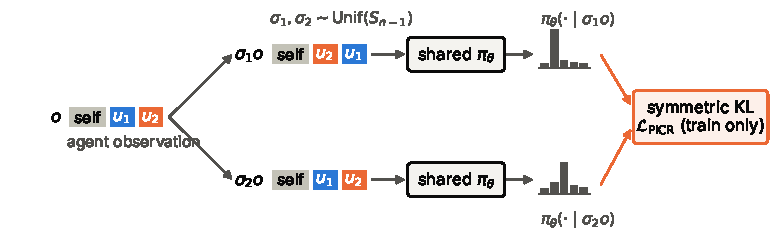
\includegraphics[width=\linewidth]{figures/method_overview.pdf}
\caption{\picr. The teammate blocks of an observation are reordered by two
independent random permutations; the shared policy is applied to both views and
the symmetric KL divergence between the two action distributions is added to the
PPO loss. The penalty is used only during training.}
\label{fig:method}
\end{figure}

\paragraph{Setting.}
We consider $n$ cooperating agents that share one policy $\pi_\theta$
(parameter sharing, \citealp{dewitt2020ippo,yu2022mappo}). Agent $i$'s
observation is $o_i = [s_i, u_{i,1}, \dots, u_{i,n-1}]$, where $s_i$ holds the
agent's own features and the environment, and $u_{i,k}$ is a fixed-width block
of features describing the $k$-th other agent (here, its relative position).
Teammates are exchangeable, so for any permutation $\sigma$ of the $n-1$ blocks
the observation $\sigma o_i = [s_i, u_{i,\sigma(1)}, \dots, u_{i,\sigma(n-1)}]$
describes the same situation. A policy is \emph{teammate-order invariant} if
$\pi_\theta(\cdot \mid \sigma o) = \pi_\theta(\cdot \mid o)$ for all $\sigma$.
An MLP over the concatenated observation has no reason to be invariant: the
slot a teammate occupies is determined by agent indices, so the policy can
learn conventions keyed to ``the first teammate''.

\paragraph{Methods.}
We compare four ways of handling teammate order, all trained with the same PPO
learner and hyperparameters:
\begin{itemize}[leftmargin=1.3em,itemsep=1pt,topsep=2pt]
\item \textbf{IPPO}: an MLP policy over $o_i$; no invariance.
\item \textbf{\picr} (Fig.~\ref{fig:method}): IPPO plus the training-time penalty
\begin{equation}
\mathcal{L}_{\picr} = \lambda\, \E_{o}\, \E_{\sigma_1,\sigma_2}
\Big[\tfrac12 \KL\big(\pi_\theta(\cdot\mid\sigma_1 o)\,\|\,\pi_\theta(\cdot\mid\sigma_2 o)\big)
   + \tfrac12 \KL\big(\pi_\theta(\cdot\mid\sigma_2 o)\,\|\,\pi_\theta(\cdot\mid\sigma_1 o)\big)\Big],
\end{equation}
with $\sigma_1, \sigma_2$ drawn uniformly and independently per observation and
gradients flowing through both views. The penalty is zero exactly when the
policy is invariant on the sampled observations; the deployed network is an
unchanged MLP.
\item \textbf{Deep Sets}: teammate blocks pass through a shared encoder and are
mean-pooled before the MLP \citep{zaheer2017deepsets}, making the policy
invariant by construction.
\item \textbf{Order augmentation}: IPPO where every policy input, during
training only, has its teammate blocks randomly permuted. For a feedforward
policy this is data augmentation over the observation symmetry. It is related
in spirit to Other-Play \citep{hu2020otherplay}, but it permutes only the
agent's view of its teammates, not the environment or the partners.
\end{itemize}

\section{Experimental protocol}
\label{sec:setup}

\paragraph{Environments.}
We use two PettingZoo MPE scenarios \citep{lowe2017maddpg,mordatch2018emergence,terry2021pettingzoo}
with three cooperating agents and 25-step episodes. In \texttt{simple\_spread}
the agents must cover three landmarks without colliding; teammate blocks hold a
teammate's relative position (and an always-zero communication channel). In
\texttt{simple\_adversary} the agents must keep an adversary, which does not
know the goal landmark, away from it, typically by sending one agent to the goal
and the others to decoy landmarks; the adversary is a separate policy trained
against the team. For speed we re-implemented both scenarios as batched NumPy
environments. They reproduce the reference \texttt{mpe2} implementation step for
step (observations, rewards and seeded resets) under identical actions, which our
test suite checks, and run about $50\times$ faster. As calibration, on our
evaluation episodes in \texttt{simple\_spread} a uniform random policy scores
\RefRandom{} and a scripted controller that uses global state to assign agents to
landmarks scores \RefAssign.

\paragraph{Learner.}
All methods use the same shared-parameter PPO learner
\citep{schulman2017ppo,dewitt2020ippo,yu2022mappo}: separate two-layer tanh MLPs
(64 units) for actor and critic, per-agent GAE
\citep{schulman2016gae} ($\gamma{=}0.99$, $\lambda_{\mathrm{GAE}}{=}0.95$), clip
0.2, entropy coefficient 0.01, Adam with learning rate $10^{-3}$, 10 epochs of 8
minibatches per update of 128 episodes, and $5\times10^{6}$ environment steps
per run. These settings were tuned for \emph{IPPO alone} on a separate tuning
seed and reused for every method (Appendix~\ref{app:tuning}), so the baseline is
at least as well tuned as the alternatives.

\paragraph{Selecting $\lambda$.}
\picr's weight was chosen per environment, by a rule fixed before any selection
run: the $\lambda \in \{0.01, 0.03, 0.1, 0.3, 1\}$ with the highest mean
cross-play on five selection seeds that are disjoint from the evaluation seeds.
This gives $\lambda=\SpreadLambda$ for \texttt{simple\_spread} and
$\lambda=\AdversaryLambda$ for \texttt{simple\_adversary}. Choosing $\lambda$ on
cross-play favours \picr{} relative to the baselines, which have no comparable
knob; it makes a negative result for \picr{} more informative, not less.

\paragraph{Zero-shot coordination.}
For each environment we train 10 independent runs (seeds 0--9) of every method
and evaluate \emph{all ordered pairs} of runs. For runs $A \neq B$, $A$'s policy
controls one agent and $B$'s policy the other two; $A=B$ is self-play. Every
pairing is scored on the same 200 evaluation episodes, whose environment seeds
are never used in training. \emph{Self-play} (SP) is the mean over runs of the
diagonal; \emph{cross-play} (XP) is the mean over ordered pairs of distinct
runs of the same method; the \emph{gap} SP$-$XP measures how much a method's
policies rely on conventions that independently trained partners do not share.
In \texttt{simple\_adversary} every team faces the same pool of adversaries,
those of all runs, assigned to episodes round-robin, so that methods are not
compared against different opponents.

\paragraph{Invariance.}
On states visited by each final policy in self-play we report the mean
Jensen--Shannon divergence between $\pi(\cdot\mid o)$ and $\pi(\cdot\mid\sigma o)$
over all non-identity permutations $\sigma$ (``perm.\ JS''; at most $\ln 2$), and
the fraction of (state, permutation) pairs on which the greedy action changes.

\paragraph{Statistics.}
Training runs are the unit of analysis \citep{henderson2018matters,agarwal2021precipice}.
We report means with 95\% percentile-bootstrap intervals over seeds; cross-play
intervals use a cluster bootstrap that resamples runs and recomputes the
all-pairs mean, because pairs sharing a run are dependent. Differences between
a method and IPPO are tested with permutation tests over run labels (10{,}000
permutations), which recompute cross-play from the full matrix of cross-method
pairings and are exact under the null hypothesis that the two methods produce
exchangeable runs.

\input{sections/results.tex}
\input{sections/discussion.tex}

\bibliographystyle{plainnat}
\bibliography{references}

\appendix
\section{Hyperparameter tuning}
\label{app:tuning}

All four methods share one PPO configuration, tuned for IPPO alone on
\texttt{simple\_spread} with a separate tuning seed (1000) and checked on
\texttt{simple\_adversary}. Selection used self-play return on the reserved
evaluation episodes. We varied the learning rate ($3{\times}10^{-4}$ to
$2{\times}10^{-3}$), epochs per update (5--15), minibatches (4--16), episodes per
update (32--256) and the entropy coefficient (0 or 0.01); the full table is in
\texttt{docs/tuning.md}. Each configuration was run with a single seed, so
differences of 1--2 return points are within seed-to-seed noise. The chosen
configuration (learning rate $10^{-3}$, 10 epochs, 8 minibatches, 128 episodes
per update, entropy 0.01) reached a training return still improving slowly at
$5\times10^{6}$ steps.

\section{Environment re-implementation}
\label{app:env}

Our batched environments follow the \texttt{mpe2} reference implementation of
\texttt{simple\_spread\_v3} (local reward ratio 0.5, agent radius 0.15, soft
contact forces) and \texttt{simple\_adversary\_v3} ($N=3$ good agents, one
adversary, shaped distance rewards), with discrete actions and 25-step
episodes. Resets reproduce the reference random-number draws exactly. The test
suite steps both implementations side by side under random actions from
several seeds and checks that observations agree to $10^{-5}$ and rewards to
$10^{-6}$ at every step. In \texttt{simple\_spread} the agents are silent, so
the two communication entries in each teammate block are always zero.

\section{Order sensitivity of the trained policies}
\label{app:sensitivity}

\begin{figure}[h]
\centering
\includegraphics[width=\linewidth]{figures/learning_curves.pdf}
\caption{Training return (top) and permutation sensitivity on the training
batch (bottom) over training; mean $\pm$ one standard error over 10 seeds. Deep
Sets is exactly invariant and is omitted from the bottom row. In
\texttt{simple\_adversary} the training return is measured against each run's
own co-trained adversary and is therefore not comparable across methods.}
\label{fig:curves}
\end{figure}

\section{Training and inference cost}
\label{app:cost}

\begin{table}[h]
\centering
\caption{Cost of one PPO update (128 episodes, 10 epochs of 8 minibatches) and
of one batched forward pass at inference time, measured in a single process on
one CPU thread on identical synthetic batches (median of 5 and 200 repeats).
\picr{} and IPPO deploy the same network. Order augmentation permutes inputs
while acting, so its update cost equals IPPO's by construction.}
\label{tab:cost}
\resizebox{\linewidth}{!}{\input{tables/overhead.tex}}
\end{table}


\end{document}
